\documentclass[english,notitlepage]{revtex4-2}  % defines the basic parameters of the document
%For preview: skriv i terminal: latexmk -pdf -pvc filnavn



% if you want a single-column, remove reprint

% allows special characters (including æøå)
\usepackage[utf8]{inputenc}
%\usepackage[english]{babel}

%% note that you may need to download some of these packages manually, it depends on your setup.
%% I recommend downloading TeXMaker, because it includes a large library of the most common packages.

\usepackage{physics,amssymb}  % mathematical symbols (physics imports amsmath)
\include{amsmath}
\usepackage{graphicx}         % include graphics such as plots
\usepackage{xcolor}           % set colors
\usepackage{hyperref}         % automagic cross-referencing (this is GODLIKE)
\usepackage{listings}         % display code
%\usepackage{subfigure}        % imports a lot of cool and useful figure commands
\usepackage{float}
%\usepackage[section]{placeins}
\usepackage{algorithm}
\usepackage[noend]{algpseudocode}
%\usepackage{subfigure}
\usepackage{tikz}
\usetikzlibrary{quantikz}
\usepackage{caption}
\usepackage{subcaption}
\usepackage{amsmath}

% defines the color of hyperref objects
% Blending two colors:  blue!80!black  =  80% blue and 20% black
\hypersetup{ % this is just my personal choice, feel free to change things
	colorlinks,
	linkcolor={red!50!black},
	citecolor={blue!50!black},
	urlcolor={blue!80!black}}

%% Defines the style of the programming listing
%% This is actually my personal template, go ahead and change stuff if you want



%% USEFUL LINKS:
%%
%%   UiO LaTeX guides:        https://www.mn.uio.no/ifi/tjenester/it/hjelp/latex/
%%   mathematics:             https://en.wikibooks.org/wiki/LaTeX/Mathematics

%%   PHYSICS !                https://mirror.hmc.edu/ctan/macros/latex/contrib/physics/physics.pdf

%%   the basics of Tikz:       https://en.wikibooks.org/wiki/LaTeX/PGF/Tikz
%%   all the colors!:          https://en.wikibooks.org/wiki/LaTeX/Colors
%%   how to draw tables:       https://en.wikibooks.org/wiki/LaTeX/Tables
%%   code listing styles:      https://en.wikibooks.org/wiki/LaTeX/Source_Code_Listings
%%   \includegraphics          https://en.wikibooks.org/wiki/LaTeX/Importing_Graphics
%%   learn more about figures  https://en.wikibooks.org/wiki/LaTeX/Floats,_Figures_and_Captions
%%   automagic bibliography:   https://en.wikibooks.org/wiki/LaTeX/Bibliography_Management  (this one is kinda difficult the first time)
%%   REVTeX Guide:             http://www.physics.csbsju.edu/370/papers/Journal_Style_Manuals/auguide4-1.pdf
%%
%%   (this document is of class "revtex4-1", the REVTeX Guide explains how the class works)


%% CREATING THE .pdf FILE USING LINUX IN THE TERMINAL
%%
%% [terminal]$ pdflatex template.tex
%%
%% Run the command twice, always.
%% If you want to use \footnote, you need to run these commands (IN THIS SPECIFIC ORDER)
%%
%% [terminal]$ pdflatex template.tex
%% [terminal]$ bibtex template
%% [terminal]$ pdflatex template.tex
%% [terminal]$ pdflatex template.tex
%%
%% Don't ask me why, I don't know.

\begin{document}
\title{Project 2}      % self-explanatory
\author{Olav K. Arnesen}          % self-explanatory
\date{\today}                             % self-explanatory
\noaffiliation                            % ignore this, but keep it.

\maketitle 

\textit{https://github.com/olavkar/fys3150/tree/main/project2}

\section*{Problem 1}
Using $\hat{x}=x/L$ means that $dx=d\hat{x}L$ and we get 
\begin{equation}
	\begin{split}
		\gamma\frac{d^2u}{dx^2}&=-Fu \\
		\rightarrow \frac{\gamma}{L^2}\frac{d^2u}{d\hat{x}^2}&=-Fu \\
		\rightarrow \frac{d^2u}{d\hat{x}^2}&= -\frac{FL^2}{\gamma}u = -\lambda u
	\end{split}
\end{equation}

\section*{Problem 2}
Running the code related to this problem confirms that armadillo agrees with the analytical solution.

\section*{Problem 3}
\subsection*{a) \& b)}
See the code related to this problem. It does indeed identify that $-0.7$ is the biggest non-diagonal element, and it gives correct indices.
	
\section*{Problem 4}
\subsection*{a) \& b)}
See code related to this problem. When comparing the eigenvalues and eigenvectors with those found in Problem 2 (by eye, in the terminal), they are in agreement.

\section*{Problem 5}
\subsection*{a)}
The number of rotations $N_{\text{rot}}$ as a function of the number of steps $N$ is shown in table \ref{tab:1}. Table \ref{tab:1} also shows how many more rotations are required from the previous $N$. This means as $N$ doubles the number of rotations approximately quadruples, suggesting $N_{\text{rot}}(N)\propto N^2$.
\begin{table} 
	\centering
	\caption{Number of rotations}
	\begin{tabular}{c@{\hspace{1cm}} c @{\hspace{1cm}}c}
		\hline
		$N$ & $N_{\text{rot}}$ & Increase \\
		\hline
		10 & 141 & - \\
		20 &  655 & 4.65 \\
		40 &  2758 & 4.21 \\
		80 & 11276 & 4.09 \\
		160 &  45595 & 4.04 \\
		\hline
	\end{tabular}\label{tab:1}
\end{table}

\subsection*{b)}
We would expect to see $N_\text{rot}=O(N^2)$ as in a), as that is approximately how many elements need to be transformed. Maybe our algorithm is about the same because non-diagonal elements, which are zero at the start, are transformed to non-zero numbers, effectively making the matrix dense.

\section*{Problem 6}
\subsection*{a) \& b)}
Figure \ref{fig:1} shows the solutions to the buckling beam problem for $n=10$ and $n=100$ steps.

\begin{figure}[h]
	\centering
	\begin{subfigure}[b]{0.95\textwidth}
		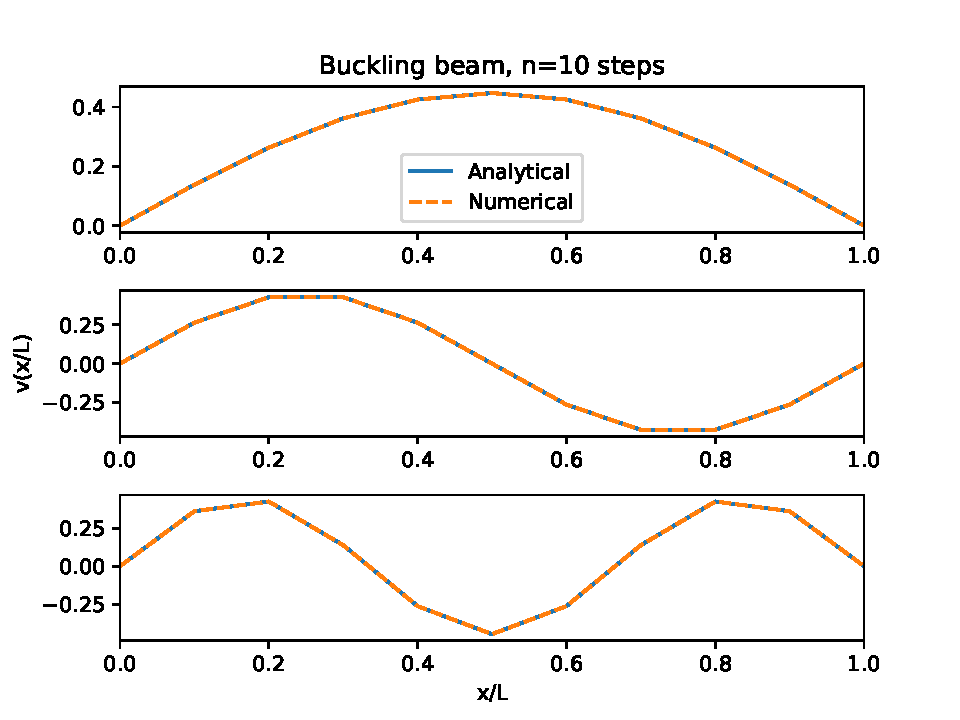
\includegraphics[scale=1]{imgs2/output_10.pdf}	
	\end{subfigure}
	\begin{subfigure}[b]{0.95\textwidth}
		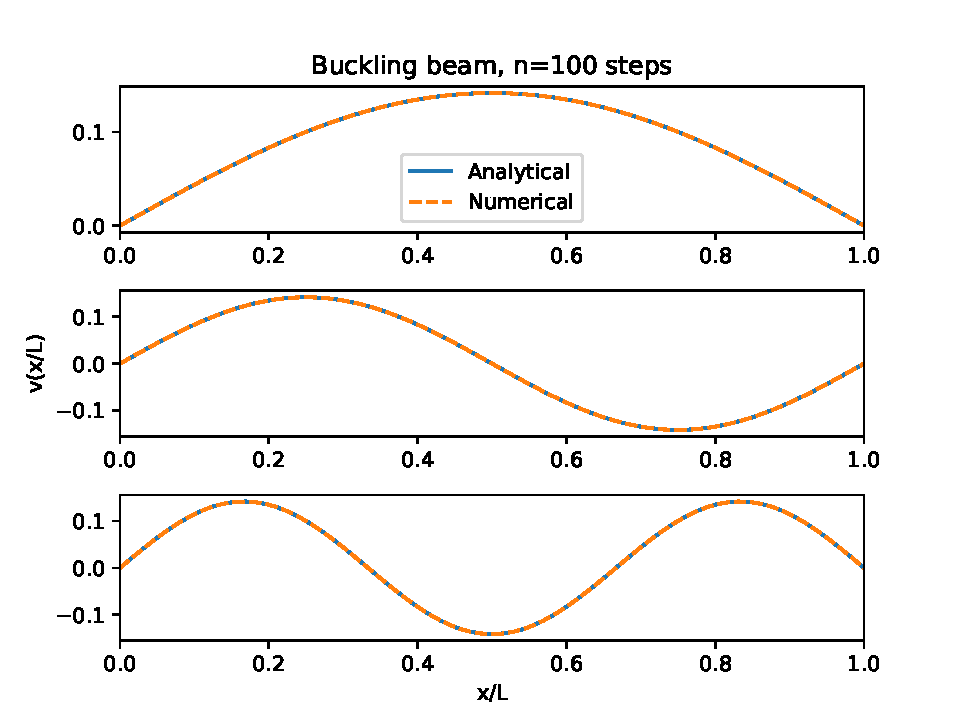
\includegraphics[scale=1]{imgs2/output_100.pdf}	
	\end{subfigure}	
	\caption{The (normalised) solutions to the buckling beam problem for the 3 lowest eigenvalues.}
	\label{fig:1}
\end{figure}

	
\end{document}